\documentclass[11pt,a4paper]{article}
\usepackage[T1]{fontenc}
\usepackage{lmodern}
\usepackage[margin=27mm]{geometry}
\usepackage{amsmath,amssymb,amsthm,mathtools}
\usepackage{microtype,booktabs,array}
\usepackage{xcolor,tikz}
\usepackage[colorlinks=true,linkcolor=blue!45!black,citecolor=blue!45!black,urlcolor=blue!45!black]{hyperref}
\hypersetup{pdftitle={Arithmetic of Ball Overlaps and Their Iterated Volume Maps},pdfauthor={KEIO},pdfsubject={Research draft: arithmetic of geometric overlaps and monomial iterations},pdfkeywords={grazing goat, Baker theorem, transcendence, ball intersection, Cantor set}}
\usepackage{fancyhdr}
\pagestyle{fancy}
\fancyhf{}
\fancyhead[L]{\small KEIO}
\fancyhead[R]{\small Arithmetic of ball overlaps}
\fancyfoot[C]{\thepage}
\setlength{\headheight}{14pt}
\setlength{\emergencystretch}{2em}
\numberwithin{equation}{section}
\newtheorem{theorem}{Theorem}[section]
\newtheorem{lemma}[theorem]{Lemma}
\newtheorem{proposition}[theorem]{Proposition}
\newtheorem{corollary}[theorem]{Corollary}
\theoremstyle{definition}
\newtheorem{definition}[theorem]{Definition}
\theoremstyle{remark}
\newtheorem{remark}[theorem]{Remark}
\newcommand{\Qbar}{\overline{\mathbb Q}}
\newcommand{\Apos}{\mathcal A}
\newcommand{\R}{\mathbb R}
\newcommand{\E}{\mathbb E}
\newcommand{\vol}{\operatorname{vol}}
\newcommand{\diam}{\operatorname{diam}}
\newcommand{\dimH}{\operatorname{dim}_{\mathrm H}}
\DeclareMathOperator{\arccosh}{arccosh}
\title{Arithmetic of Ball Overlaps\texorpdfstring{\\}{ }and Their Iterated Volume Maps}
\author{KEIO}
\date{12 October 2026\\[3pt]\small Research draft}

\begin{document}
\maketitle
\begin{abstract}
The grazing-goat problem asks for the radius of a ball that covers a prescribed fraction of another ball. We prove a parity theorem for genuine partial overlaps with algebraic radii and algebraic centre distance: the normalized intersection volume is algebraic in odd dimension and transcendental in even dimension. A positive algebraic correction in the spherical-cap formula makes Baker's theorem applicable. This gives a complete classification of the inverse problem for algebraic target fractions and algebraic anchor distances, including its containment exceptions. For the boundary half-volume constants $\alpha_n$, we establish strict increase along each parity subsequence and a third-order asymptotic expansion; the three-dimensional constant has degree four and Galois group $S_4$. We then study a separate iteration obtained by reinterpreting dimensionless overlap volumes as radii. For a general class of monomial maps, at most one finite path from any positive starting value can have an algebraic output. We classify all exceptional starting values and all coincidences of periodic radii. For the two- and three-dimensional overlap maps, the periodic radii are transcendental and their closure is the exponential image of a self-similar Cantor set of dimension determined by $2^{-s}+3^{-s}=1$.
\end{abstract}
\noindent\textbf{Keywords.} Ball intersection; grazing-goat problem; Baker's theorem; algebraic numbers; monomial semigroups; self-similar sets.

\section{Introduction}

Let $B_n(c,R)$ be the closed Euclidean ball with centre $c\in\R^n$ and radius $R>0$, and let $\omega_n=\vol B_n(0,1)$. The classical boundary grazing problem defines $\alpha_n$ by
\begin{equation}\label{eq:alpha-def}
 \vol\bigl(B_n(0,1)\cap B_n(e_1,\alpha_n)\bigr)=\frac{\omega_n}{2}.
\end{equation}
Thus a pasture of radius $R$ requires rope length $R\alpha_n$. The planar problem and its higher-dimensional versions have an established literature, including Fraser \cite{Fraser} and Meyerson \cite{Meyerson}. The planar and spatial constants also appear in the OEIS \cite{OEIS2,OEIS3}. Our aim is to organize arithmetic consequences of the cap formulas and then investigate a distinct iteration suggested by the same geometry.

There are two constructions in this paper. In the \emph{inverse overlap problem}, a volume fraction is prescribed and the radius is solved for. In the \emph{iterated volume problem}, equal-radius overlap volumes are first made dimensionless and their numerical values are used as new radii. They lead to different maps: the first scales a physical radius by $\alpha_n$, whereas the second produces monomials such as $Cx^2$ and $Dx^3$. Keeping this distinction explicit is essential.

The central geometric result is stronger than the half-volume problem. If two balls have algebraic radii and algebraic centre distance and form a genuine partial overlap, then their intersection fraction is algebraic in odd dimension and transcendental in even dimension. The even-dimensional proof combines Baker's theorem with a positivity lemma valid even when one of the two caps is larger than a hemisphere. The inverse classification follows for every algebraic target fraction in $(0,1)$ and every algebraic anchor distance.

The second group of results concerns maps $T_i(x)=c_i x^{d_i}$ whose coefficients are multiplicatively independent modulo algebraic numbers. A weighted exponent identity and a decoding argument show that a starting value has at most one algebraic finite-path output. We obtain the exact exceptional sets, transcendence of every positive periodic radius, and a classification of coincidences by primitive words. The geometric pair $C=2\pi/3-\sqrt3/2$, $D=5\pi/12$ also produces an explicit Cantor closure of periodic radii.

We provide proofs of the statements used here and distinguish them from established geometric formulas and constants. The Hall--Tenenbaum connection discussed below is already recorded in the literature. This draft does not claim a proof of irrationality or transcendence of Euler's constant, the Euler--Gompertz constant, or Catalan's constant. Historical priority for the individual extensions is not established by the present literature review.

\section{Arithmetic of partial ball overlaps}\label{sec:lenses}

For $-1<s<1$, define the cap integral
\begin{equation}\label{eq:cap}
 J_n(s)=\int_s^1(1-u^2)^{(n-1)/2}\,du.
\end{equation}
Write
\[
 Q_n(r,d)=\frac{\vol\bigl(B_n(0,1)\cap B_n(de_1,r)\bigr)}{\omega_n}.
\]
A \emph{genuine partial overlap} means
\begin{equation}\label{eq:partial}
 r>0,\quad d>0,\quad |1-r|<d<1+r.
\end{equation}
In this case set
\begin{equation}\label{eq:cuts}
 t=\frac{1+d^2-r^2}{2d},\qquad
 x=\frac{d^2+r^2-1}{2dr},\qquad
 h=\sqrt{1-t^2}=r\sqrt{1-x^2}.
\end{equation}
Then $-1<t,x<1$, $h>0$, and $t+rx=d$. Slicing the lens at its common boundary plane gives
\begin{equation}\label{eq:lens}
 Q_n(r,d)=\frac{J_n(t)+r^nJ_n(x)}{2J_n(0)},
\end{equation}
because $\omega_n=2\omega_{n-1}J_n(0)$, with $\omega_0=1$.

\begin{figure}[ht]
\centering
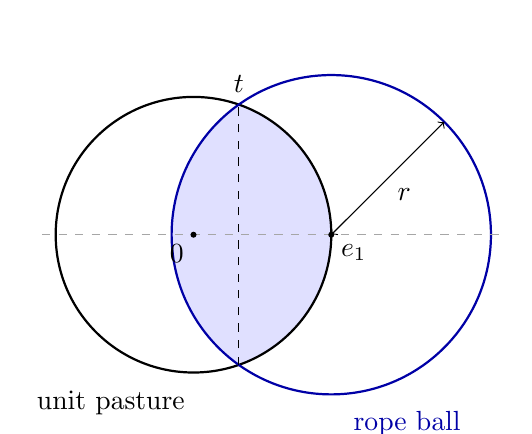
\begin{tikzpicture}[scale=1.75]
 \begin{scope}
  \clip (0,0) circle (1);
  \fill[blue!12] (1,0) circle (1.158728473);
 \end{scope}
 \draw[thick] (0,0) circle (1);
 \draw[thick,blue!65!black] (1,0) circle (1.158728473);
 \draw[gray!70,dashed] (-1.1,0)--(2.25,0);
 \draw[dashed] (.328674,-.944443)--(.328674,.944443);
 \fill (0,0) circle (.022) node[below left] {$0$};
 \fill (1,0) circle (.022) node[below right] {$e_1$};
 \draw[<->] (1,0)--(1.82,.8187) node[midway,below right] {$r$};
 \node[above] at (.328674,.96) {$t$};
 \node at (-.6,-1.22) {unit pasture};
 \node[blue!65!black] at (1.55,-1.37) {rope ball};
\end{tikzpicture}
\caption{The boundary case $d=1$ in a two-dimensional cross-section. The common cut has coordinate $t=1-r^2/2$; measured from the rope-ball centre and divided by $r$, its opposite coordinate is $x=r/2$.}
\label{fig:lens}
\end{figure}

We use the following standard consequence of Baker's theorem \cite{Baker}: if $\eta_1,\ldots,\eta_k$ are nonzero algebraic numbers, fixed values of their logarithms are chosen, and $b_1,\ldots,b_k$ are algebraic, then
\begin{equation}\label{eq:baker}
 b_1\log\eta_1+\cdots+b_k\log\eta_k
 \quad\text{is either zero or transcendental.}
\end{equation}

\begin{lemma}[Positive cap correction]\label{lem:positive}
For $m\geq1$, put
\[
 c_m=\binom{2m}{m}4^{-m},\qquad
 P_{m-1}(z)=\sum_{k=1}^m\frac{z^{k-1}}{2k c_k}.
\]
Then
\begin{equation}\label{eq:even-cap}
 J_{2m}(s)=c_m\arccos s-E_m(s),\qquad
 E_m(s)=c_m s\sqrt{1-s^2}\,P_{m-1}(1-s^2).
\end{equation}
For every genuine partial overlap, the combined correction satisfies
\begin{equation}\label{eq:positive}
 A:=E_m(t)+r^{2m}E_m(x)>0.
\end{equation}
\end{lemma}
\begin{proof}
Integration by parts gives
\[
 J_{2m}(s)=\frac{2m-1}{2m}J_{2m-2}(s)
 -\frac{s(1-s^2)^{m-1/2}}{2m}.
\]
Starting with the auxiliary integral $J_0(s)=\arccos s$ and iterating proves \eqref{eq:even-cap}. All coefficients of $P=P_{m-1}$ are positive. Consequently
\begin{equation}\label{eq:poly-bound}
 P(az)\leq a^{m-1}P(z)\qquad(a\geq1,\ z\geq0).
\end{equation}
Let $H=h^2$. The identities in \eqref{eq:cuts} give
\[
 \frac{A}{c_mh}=tP(H)+r^{2m-1}xP(H/r^2).
\]
If $t,x\geq0$, this is positive since $t+rx=d>0$. They cannot both be negative. If $t<0$, then $r>1$ and $x>0$. By \eqref{eq:poly-bound}, $P(H)\leq r^{2m-2}P(H/r^2)$; multiplying by the negative number $t$ yields
\[
 \frac{A}{c_mh}\geq r^{2m-2}(t+rx)P(H/r^2)>0.
\]
If $x<0$, then $r<1$ and $t>0$. Now $P(H/r^2)\leq r^{-2m+2}P(H)$, so
\[
 \frac{A}{c_mh}\geq (t+rx)P(H)>0.
\]
These cases prove the assertion.
\end{proof}

\begin{theorem}[Parity theorem for algebraic lenses]\label{thm:lens}
Suppose that two balls have positive algebraic radii and positive algebraic centre distance and form a genuine partial overlap. Their intersection volume divided by the volume of either ball is algebraic in odd dimension and transcendental in even dimension.
\end{theorem}
\begin{proof}
Scale the first radius to $1$. The normalized radius $r$ and centre distance $d$ remain algebraic. If $n=2m+1$, the integrand of $J_n$ is a polynomial with rational coefficients. Hence $J_n$ is such a polynomial, and \eqref{eq:lens} is algebraic.

Let $n=2m$ and suppose, for a contradiction, that $q=Q_{2m}(r,d)$ is algebraic. Since $2J_{2m}(0)=c_m\pi$, equations \eqref{eq:lens} and \eqref{eq:even-cap} imply
\[
 \arccos t+r^{2m}\arccos x-q\pi=A/c_m.
\]
Here $A$ is a positive algebraic number by Lemma~\ref{lem:positive}. For $-1<s<1$, use the principal logarithm identity
\[
 \log\bigl(s+i\sqrt{1-s^2}\bigr)=i\arccos s,
 \qquad \log(-1)=i\pi.
\]
Multiplying the preceding equation by $i$ gives a linear form in logarithms of nonzero algebraic numbers, with algebraic coefficients, equal to the nonzero algebraic number $iA/c_m$. This contradicts \eqref{eq:baker}. The fraction relative to the second ball is $q/r^n$, so the same arithmetic type holds for it.
\end{proof}

\begin{theorem}[Complete inverse classification]\label{thm:inverse}
Let $d\geq0$ and $q\in(0,1)$ be algebraic real numbers. There is a unique $r>0$ such that $Q_n(r,d)=q$. For odd $n$, this radius is algebraic. For even $n$, it is algebraic precisely in the following containment cases:
\begin{equation}\label{eq:containment}
 d=0,\qquad\text{or}\qquad 0<d<1\ \text{and}\ q\leq(1-d)^n.
\end{equation}
In these cases $r=q^{1/n}$. In every other even-dimensional case, $r$ is transcendental.
\end{theorem}
\begin{proof}
The function $r\mapsto Q_n(r,d)$ is continuous, is zero up to the first contact, and is one for $r\geq d+1$. It is strictly increasing whenever its value lies between zero and one: every nonempty radial shell in this range intersects the interior of the unit ball in a nonempty open set. This proves existence and uniqueness for $0<q<1$.

For $d=0$, $Q_n(r,0)=\min(1,r^n)$. If $0<d<1$ and $r\leq1-d$, the smaller ball is contained in the unit ball, so $Q_n(r,d)=r^n$. These are exactly the cases in \eqref{eq:containment}, including the internal tangency at equality. All remaining solutions form genuine partial overlaps. For even $n$, an algebraic $r$ would contradict Theorem~\ref{thm:lens}.

For odd $n$, $J_n$ is a polynomial of degree $n$ over $\mathbb Q$. With $d>0$ fixed and algebraic, $t(r)$ is a polynomial in $r^2$ over $\Qbar$, while $x(r)=(d^2+r^2-1)/(2dr)$. Each $r^n x(r)^j$, $0\leq j\leq n$, is a polynomial in $r$. Therefore
\[
 J_n(t(r))+r^nJ_n(x(r))-2qJ_n(0)=0
\]
is a polynomial equation over $\Qbar$. Its polynomial is not identically zero, since $Q_n(r,d)$ is strictly increasing on the partial-overlap interval. Its root $r$ is consequently algebraic.
\end{proof}

\begin{corollary}[Boundary and exterior anchors]\label{cor:boundary}
For every algebraic $d\geq1$ and every algebraic $q\in(0,1)$, the unique normalized rope length is algebraic in odd dimension and transcendental in even dimension.
\end{corollary}

The partial-overlap hypothesis in Theorem~\ref{thm:lens} is necessary. For contained balls with algebraic radii, the normalized volume is a power of an algebraic radius in every dimension. Likewise the restrictions $0<q<1$ in Theorem~\ref{thm:inverse} exclude the nonunique endpoint problems.

\section{Boundary half-volume constants}\label{sec:half}

At $d=1$, the half-volume equation \eqref{eq:alpha-def} becomes
\begin{equation}\label{eq:half}
 r^nJ_n(r/2)+J_n(1-r^2/2)=J_n(0),\qquad 0<r<2.
\end{equation}
Its unique solution is $\alpha_n$. In dimension one the pasture is the interval $[-1,1]$ with tether at $1$, and hence $\alpha_1=1$.

\begin{proposition}\label{prop:bounds}
For every $n\geq2$, $1<\alpha_n<\sqrt2$. The number $\alpha_n$ is algebraic for odd $n$ and transcendental for even $n$.
\end{proposition}
\begin{proof}
The arithmetic statement follows from Corollary~\ref{cor:boundary}. If a point $X$ in the unit ball is reached by rope length $1$, then $\|X\|^2\leq2X_1$. For $n\geq2$, this is a proper subset of positive-measure complement in the half-ball $X_1\geq0$. Thus the reached volume is less than one half.

For length $\sqrt2$, the condition is $X_1\geq(\|X\|^2-1)/2$. It contains the positive half-ball and an open set on the negative side. Thus the reached volume is greater than one half. Strict monotonicity in $r$ gives the bounds.
\end{proof}

\subsection{The spatial constant and its Galois group}

For $n=3$, $J_3(s)=2/3-s+s^3/3$, so direct substitution yields
\begin{equation}\label{eq:spatial}
 Q_3(r,1)=\frac{r^3(8-3r)}{16},\qquad
 3\alpha_3^4-8\alpha_3^3+8=0.
\end{equation}
This quartic and its numerical root are recorded in \cite{OEIS3}.

\begin{proposition}\label{prop:s4}
The algebraic number $\alpha_3$ has degree four over $\mathbb Q$. Its splitting field has Galois group $S_4$, and $\alpha_3$ is not constructible by straightedge and compass.
\end{proposition}
\begin{proof}
Put $u=2/\alpha_3$. Equation \eqref{eq:spatial} becomes
\[
 f(u)=0,\qquad f(X)=X^4-8X+6.
\]
The polynomial $f$ is Eisenstein at $2$, hence irreducible. The fields $\mathbb Q(u)$ and $\mathbb Q(\alpha_3)$ are equal, giving degree four. The discriminant is
\[
 \operatorname{disc}(f)=256\cdot6^3-27\cdot8^4=-55296=-6\cdot96^2,
\]
which is not a square. Modulo $5$,
\[
 f(X)=(X-4)(X^3+4X^2+X+1).
\]
The cubic has no root in $\mathbb F_5$, so it is irreducible there. Since $5$ does not divide the discriminant, this factorization shows that the Galois group contains a $3$-cycle. A transitive subgroup of $S_4$ with a $3$-cycle is $A_4$ or $S_4$, and the nonsquare discriminant excludes $A_4$. The roots of the quartic in \eqref{eq:spatial} and those of $f$ correspond by $z\mapsto2/z$, so their splitting fields coincide. A constructible algebraic number has a normal closure of degree a power of $2$. The group $S_4$ has order $24$, proving nonconstructibility.
\end{proof}

This does not preclude an expression by radicals: $S_4$ is solvable. It precludes an expression using only rational operations and successive square roots. In particular, degree four by itself would not have been enough to decide constructibility.

For comparison, the next two odd-dimensional equations are
\begin{align}
 5\alpha_5^8-80\alpha_5^6+128\alpha_5^5-128&=0,\label{eq:n5}\\
 7\alpha_7^{12}-112\alpha_7^{10}+840\alpha_7^8-1024\alpha_7^7+1024&=0.
\end{align}
These identities assert algebraicity, not irreducibility or minimal degree.

\subsection{The Hall--Tenenbaum constant}

The Hall--Tenenbaum constant $\kappa$ occurs in bounds for mean values of multiplicative functions \cite{HallTenenbaum}. A defining parametrization is
\begin{equation}\label{eq:hall}
 \kappa=-\cos\psi,\qquad
 \sin\psi-\psi\cos\psi=\frac\pi2,\qquad 0<\psi<\pi.
\end{equation}
The function on the left has derivative $\psi\sin\psi>0$, so this parameter is unique. Its connection with the planar grazing constant is already documented in \cite{OEISPsi,Finch}:
\begin{equation}\label{eq:hall-goat}
 \alpha_2=2\cos(\psi/2),\qquad
 \kappa=1-\frac{\alpha_2^2}{2}
 =0.3286741629085462168\ldots.
\end{equation}
Indeed, substituting $r=2\cos(\psi/2)$ in \eqref{eq:half} for $n=2$ gives exactly \eqref{eq:hall}.

\begin{corollary}\label{cor:hall}
The number $\kappa$ defined by \eqref{eq:hall} is transcendental.
\end{corollary}
\begin{proof}
If $\kappa$ were algebraic, \eqref{eq:hall-goat} would make $\alpha_2$ algebraic, contradicting Proposition~\ref{prop:bounds}.
\end{proof}

There is also a short direct Baker argument, illustrating that geometry is not required for this consequence. If $\kappa$ were algebraic, set $z=\kappa+i\sqrt{1-\kappa^2}$. Since $\arccos\kappa=\pi-\psi$, equation \eqref{eq:hall} implies
\[
 (1/2-\kappa)\log(-1)+\kappa\log z=i\sqrt{1-\kappa^2}.
\]
The right side would be nonzero and algebraic, contradicting \eqref{eq:baker}. We make no claim of historical priority for this application.

\subsection{Scaling and arithmetic transfer}

For a pasture of radius $R>0$, boundary tether, and half-volume target, the rope length is
\begin{equation}\label{eq:scaling}
 L_n(R)=R\alpha_n.
\end{equation}
For odd $n$, multiplication by the nonzero algebraic number $\alpha_n$ preserves algebraicity and transcendence:
\begin{equation}\label{eq:transfer}
 R\in\Qbar\quad\Longleftrightarrow\quad L_n(R)\in\Qbar.
\end{equation}
This equivalence does not preserve rationality: multiplication by an algebraic irrational can turn another algebraic irrational into a rational number. For even $n$, an algebraic nonzero $R$ gives a transcendental $L_n(R)$, but no such conclusion follows for an arbitrary transcendental $R$. For example, $R=1/\alpha_n$ gives $L_n(R)=1$.

In particular, choosing $R=\gamma$ (Euler's constant) or
\[
 R=\delta:=\int_0^\infty\frac{e^{-t}}{1+t}\,dt
 \quad\text{(the Euler--Gompertz constant)}
\]
does not settle the arithmetic nature of that starting constant. In odd dimension \eqref{eq:transfer} returns the same algebraicity question; in even dimension an additional independent relation would be needed.

\section{Dimension growth and an asymptotic expansion}\label{sec:asymptotic}

\begin{theorem}[Monotonicity along each parity subsequence]\label{thm:monotone}
For every integer $n\geq1$, $\alpha_{n+2}>\alpha_n$.
\end{theorem}
\begin{proof}
Integration by parts in \eqref{eq:cap} gives
\begin{equation}\label{eq:dimension-recurrence}
 J_{n+2}(s)=\frac{n+1}{n+2}J_n(s)
 -\frac{s(1-s^2)^{(n+1)/2}}{n+2}.
\end{equation}
Put $r=\alpha_n$, $a=r/2$, and $b=1-r^2/2$. Then $1-b^2=r^2(1-a^2)$ and $ra+b=1$. Substituting \eqref{eq:dimension-recurrence} into the half-volume residual in dimension $n+2$ and using \eqref{eq:half} gives
\begin{align*}
 &r^{n+2}J_{n+2}(a)+J_{n+2}(b)-J_{n+2}(0)\\
 &\qquad=\frac{r^n}{n+2}
 \left[(n+1)(r^2-1)J_n(a)-r(1-a^2)^{(n+1)/2}\right].
\end{align*}
For $0<a<1$,
\[
 J_n(a)<\frac1a\int_a^1u(1-u^2)^{(n-1)/2}\,du
 =\frac{(1-a^2)^{(n+1)/2}}{(n+1)a}.
\]
When $n\geq2$, Proposition~\ref{prop:bounds} gives $1<r<\sqrt2$. The bracket above is therefore strictly less than
\[
 \left(\frac{r^2-1}{a}-r\right)(1-a^2)^{(n+1)/2}
 =\frac{r^2-2}{r}(1-a^2)^{(n+1)/2}<0.
\]
For $n=1$, $r=1$ makes the bracket negative directly. Thus radius $\alpha_n$ reaches less than half the volume in dimension $n+2$. Uniqueness and monotonicity in the radius prove the result.
\end{proof}

\begin{theorem}[Third-order expansion]\label{thm:asymptotic}
As $n\to\infty$,
\begin{align}
 \alpha_n^2&=2-\frac2n+\frac{8}{3n^2}-\frac{128}{15n^3}+O(n^{-4}),\label{eq:alpha-square-asympt}\\
 \alpha_n&=\sqrt2\left(1-\frac1{2n}+\frac{13}{24n^2}-\frac{149}{80n^3}+O(n^{-4})\right).\label{eq:alpha-asympt}
\end{align}
In particular, both parity subsequences converge to $\sqrt2$, and
\[
 n(\sqrt2-\alpha_n)\longrightarrow\frac1{\sqrt2}.
\]
\end{theorem}
\begin{proof}
Let $X$ be uniform in the unit ball and write $X=RU$, where $U$ is uniform on the unit sphere and independent of $R$. Since $\Pr(R\leq r)=r^n$, we may represent
\[
 R=e^{-Y/n},\qquad Y\sim\operatorname{Exp}(1)
\]
exactly. For $n\geq3$, the first coordinate of $U$ has density $b_n(1-u^2)^{(n-3)/2}$ on $(-1,1)$, where $b_n$ is a normalizing constant. Define the odd, saturated integral
\[
 K_n(t)=\int_0^{\max(-1,\min(1,t))}(1-u^2)^{(n-3)/2}\,du.
\]
For a proposed squared radius $2-h$, the reach condition is
\[
 U_1\geq t_n(Y,h),\qquad
 t_n(Y,h)=-\sinh(Y/n)+\frac h2e^{Y/n}.
\]
Its probability is $1/2-b_n\Phi_n(h)$, with
\[
 \Phi_n(h)=\E K_n(t_n(Y,h)).
\]
Thus $h_n=2-\alpha_n^2$ is the unique zero corresponding to $0<\alpha_n<2$.

For fixed bounded $A,B,C$ and $h=A/n+B/n^2+C/n^3$, expansion gives
\[
 t_n=\frac vn+\frac w{n^2}+\frac z{n^3}
 +O\bigl((1+Y)^4n^{-4}\bigr),
\]
where
\[
 v=A/2-Y,\quad w=B/2+AY/2,\quad
 z=C/2+BY/2+AY^2/4-Y^3/6.
\]
The centered integral has the expansion
\[
 K_n(t)=t-\frac{n-3}{6}t^3
 +\frac{(n-3)(n-5)}{40}t^5+O(n^3|t|^7).
\]
To justify averaging these expansions, first restrict to $0\leq Y\leq n^{1/10}$. There $n t_n^2\to0$ uniformly and the displayed remainders have uniform bounds. Exponential moments of every fixed polynomial in $Y$ are finite. On the complement, $|K_n|\leq1$, and the exponential tail and polynomial moment tails are smaller than every inverse power of $n$. The averaged remainder is consequently $O(n^{-4})$.

Collecting terms yields
\begin{align}\label{eq:phi-expansion}
 \Phi_n(h)={}&\frac{\E v}{n}
 +\frac{\E w-\E(v^3)/6}{n^2}\notag\\
 &+\frac{\E z-\E(v^2w)/2+\E(v^3)/2+\E(v^5)/40}{n^3}
 +O(n^{-4}).
\end{align}
Using $\E Y^j=j!$, the first coefficient vanishes for $A=2$. The second then equals $B/2+4/3$, so $B=-8/3$. At these values,
\[
 \E v^3=-2,\qquad \E(v^2w)=5/3,\qquad
 \E v^5=-44,\qquad \E z=C/2-4/3.
\]
The third coefficient is $C/2-64/15$, giving $C=128/15$. Therefore
\[
 h_*:=\frac2n-\frac8{3n^2}+\frac{128}{15n^3}
 \quad\text{satisfies}\quad \Phi_n(h_*)=O(n^{-4}).
\]

It remains to pass from a residual estimate to the actual root. The leading term in \eqref{eq:phi-expansion} gives opposite signs at $h=1/n$ and $h=3/n$, so $h_n$ lies between them for large $n$. On this interval, for $0\leq Y\leq1$, $|t_n|=O(1/n)$ and
\[
 \frac{\partial}{\partial h}K_n(t_n(Y,h))
 =\frac12e^{Y/n}(1-t_n(Y,h)^2)^{(n-3)/2}
\]
has a uniform positive lower bound. All other contributions are nonnegative, since $K_n(t_n(Y,h))$ is nondecreasing in $h$. Integrating the resulting finite-difference inequality gives a constant $c>0$, independent of large $n$, such that
\[
 \Phi_n(h')-\Phi_n(h)\geq c(h'-h)
 \quad(1/n\leq h<h'\leq3/n).
\]
It follows that $|h_n-h_*|=O(n^{-4})$. Subtracting from $2$ proves \eqref{eq:alpha-square-asympt}; expansion of the positive square root gives \eqref{eq:alpha-asympt}.
\end{proof}

The limit $\sqrt2$ belongs to the earlier geometric study \cite{Fraser,Meyerson}; the proof above records explicit correction terms. Theorem~\ref{thm:asymptotic} also gives $\alpha_{n+1}>\alpha_n$ for all sufficiently large $n$. Theorem~\ref{thm:monotone} asserts a global comparison two dimensions apart; a global adjacent-dimensional comparison is not proved here.

\begin{table}[ht]
\centering
\caption{Boundary half-volume radii. Values are rounded to 12 decimal places; the arithmetic classification is proved independently of these computations.}
\label{tab:alpha}
\begin{tabular}{rll}
\toprule
$n$ & $\alpha_n$ & Arithmetic type established here\\
\midrule
1 & 1.000000000000 & rational\\
2 & 1.158728473018 & transcendental\\
3 & 1.228544863735 & algebraic of degree 4; not constructible\\
4 & 1.268079256673 & transcendental\\
5 & 1.293597996360 & algebraic\\
6 & 1.311461819027 & transcendental\\
7 & 1.324679635868 & algebraic\\
8 & 1.334862429158 & transcendental\\
9 & 1.342951798535 & algebraic\\
10 & 1.349535439998 & transcendental\\
50 & 1.400359338024 & transcendental\\
100 & 1.407216638715 & transcendental\\
200 & 1.410696861483 & transcendental\\
\bottomrule
\end{tabular}
\end{table}

\section{From overlap volumes to monomial maps}\label{sec:maps}

Consider two balls of equal radius $R$ whose centres are distance $R$ apart. Their overlap area in dimension two and volume in dimension three are respectively
\begin{equation}\label{eq:CD}
 CR^2,\qquad DR^3,\qquad
 C=\frac{2\pi}{3}-\frac{\sqrt3}{2},\qquad D=\frac{5\pi}{12}.
\end{equation}
For example, the planar intersection is twice the unit cap of opening angle $2\pi/3$, scaled by $R^2$, giving $C$. In three dimensions, \eqref{eq:spatial} at $r=1$ gives fraction $5/16$ of a ball of volume $4\pi R^3/3$, giving $D$.

Areas and volumes cannot be substituted directly for physical lengths. Fix a reference length $L_0>0$ and write $x=R/L_0$. Divide the area by $L_0^2$ or the volume by $L_0^3$, respectively. Reinterpreting these dimensionless numbers as the next dimensionless radius defines
\begin{equation}\label{eq:FG}
 F(x)=Cx^2,\qquad G(x)=Dx^3,\qquad x>0.
\end{equation}
This is a specified numerical iteration, dependent on the chosen normalization. It is distinct from the half-volume rope map \eqref{eq:scaling}.

\begin{lemma}[Multiplicative independence modulo algebraic numbers]\label{lem:CD}
For $u,v\in\mathbb Z$,
\begin{equation}\label{eq:CD-independent}
 C^uD^v\in\Qbar\quad\Longrightarrow\quad u=v=0.
\end{equation}
\end{lemma}
\begin{proof}
Put $\beta=3\sqrt3/4$. Then $C=(2/3)(\pi-\beta)$ and $D=(5/12)\pi$. If $C^uD^v$ is algebraic, the rational function
\[
 R(X)=(X-\beta)^uX^v\in\Qbar(X)
\]
has algebraic value at $X=\pi$. The orders of its zeros or poles at $\beta$ and $0$ are $u$ and $v$, respectively, so $R$ is constant only if $u=v=0$. Otherwise, writing $R=P/Q$, an algebraic value $R(\pi)=a$ gives the nonzero polynomial equation $P(\pi)-aQ(\pi)=0$ over $\Qbar$. This would make $\pi$ algebraic, a contradiction.
\end{proof}

The coefficients $C,D$ are not algebraically independent; both are affine expressions in $\pi$. Lemma~\ref{lem:CD} states only the multiplicative independence needed below.

\subsection{A general semigroup theorem}

Let $k\geq1$, let $d_1,\ldots,d_k$ be integers at least $2$, and let $c_1,\ldots,c_k$ be positive real numbers. Assume
\begin{equation}\label{eq:MI}
 \prod_{i=1}^k c_i^{u_i}\in\Qbar,\quad u_i\in\mathbb Z
 \quad\Longrightarrow\quad u_1=\cdots=u_k=0.
\end{equation}
Set $T_i(x)=c_i x^{d_i}$. A finite word $w=i_1\cdots i_\ell$ is read in chronological order:
\[
 T_w=T_{i_\ell}\circ\cdots\circ T_{i_1}.
\]
The empty word $\varnothing$ represents the identity. There are integers $a_i(w)\geq0$ and $N(w)\geq1$ such that
\begin{equation}\label{eq:word-form}
 T_w(x)=c^{a(w)}x^{N(w)},\qquad
 c^a:=\prod_{i=1}^k c_i^{a_i},\qquad
 N(w)=\prod_{j=1}^{\ell}d_{i_j}.
\end{equation}
For the empty word, $a=0$ and $N=1$.

\begin{lemma}[Invariant and decoding]\label{lem:encoding}
Every finite word satisfies
\begin{equation}\label{eq:invariant}
 \sum_{i=1}^k(d_i-1)a_i(w)=N(w)-1.
\end{equation}
Moreover, the pair $(a(w),N(w))$ determines the word uniquely.
\end{lemma}
\begin{proof}
Appending a letter $i$ as the final operation changes
\[
 (a,N)\longmapsto(d_i a+e_i,d_iN),
\]
where $e_i$ is the $i$th coordinate vector. This preserves \eqref{eq:invariant}, which holds for the empty word.

For a nonempty word whose first letter is $i$, the contribution of that first operation to $a_i$ is $N/d_i$, because every later degree multiplies its exponent. Hence
\[
 \frac{(d_i-1)a_i}{N}\geq\frac{d_i-1}{d_i}\geq\frac12.
\]
The sum of these normalized coordinates is $1-1/N<1$, so there can be only one coordinate at least $1/2$. It identifies the first letter. Removing that letter leaves the data
\[
 N'=N/d_i,\qquad a'=a-(N/d_i)e_i
\]
for the suffix word. Repeat until $N=1$, which identifies the empty word. This proves unique decoding.
\end{proof}

\begin{theorem}[At most one algebraic path]\label{thm:one-path}
Under \eqref{eq:MI}, for every $R>0$ at most one finite word $w$, including the empty word, has $T_w(R)\in\Qbar$.
\end{theorem}
\begin{proof}
Suppose that $U=T_w(R)=c^aR^N$ and $V=T_v(R)=c^bR^M$ are both algebraic. They are positive, so
\[
 U^M/V^N=c^{Ma-Nb}\in\Qbar.
\]
Assumption \eqref{eq:MI} gives $Ma_i=Nb_i$ for each $i$. Taking the weighted sum in \eqref{eq:invariant} gives
\[
 M(N-1)=N(M-1),
\]
so $M=N$ and $a=b$. Lemma~\ref{lem:encoding} gives $w=v$.
\end{proof}

\begin{corollary}[Faithful word representation]\label{cor:faithful}
Distinct finite words define distinct functions on $(0,\infty)$.
\end{corollary}
\begin{proof}
Equality of the positive monomial functions gives equality of degrees and coefficients. By \eqref{eq:MI}, the coefficient exponents agree; Lemma~\ref{lem:encoding} then makes the words equal.
\end{proof}

\subsection{Exact exceptional sets}

Let $\Apos=\Qbar\cap(0,\infty)$, a countable dense multiplicative group. For each finite word define
\begin{equation}\label{eq:exceptional}
 E_w=(c^{a(w)})^{-1/N(w)}\Apos.
\end{equation}

\begin{theorem}[Classification of algebraic outputs]\label{thm:exceptional}
The sets $E_w$ are pairwise disjoint, and
\begin{equation}\label{eq:equivalence-E}
 T_w(R)\in\Qbar\quad\Longleftrightarrow\quad R\in E_w.
\end{equation}
Each $E_w$ is countable and dense in $(0,\infty)$. The empty-word set is $E_{\varnothing}=\Apos$; every nonempty-word set consists entirely of transcendental numbers. The union
\[
 E=\bigcup_w E_w
\]
is countable and dense. Every $R\in E$ has exactly one algebraic path output, and every $R\notin E$ has none. In particular, outside a set of Lebesgue measure zero and first category, all finite-path outputs are transcendental.
\end{theorem}
\begin{proof}
Positive integer powers and positive integer roots map $\Apos$ onto itself. Solving $c^aR^N\in\Apos$ therefore gives exactly \eqref{eq:exceptional}, proving \eqref{eq:equivalence-E}. Pairwise disjointness follows from Theorem~\ref{thm:one-path}. Each set is a positive scalar multiple of the countable dense set $\Apos$, so it is countable and dense. A nonempty-word set is disjoint from $E_{\varnothing}=\Apos$, and thus contains no algebraic numbers. There are countably many finite words. Hence $E$ is countable, dense, null, and meagre; its complement has the stated properties.
\end{proof}

For the geometric maps \eqref{eq:FG}, Lemma~\ref{lem:CD} supplies \eqref{eq:MI}. Thus, for any positive starting value, all but at most one of the indexed expressions
\[
 R,\quad F(R),\quad G(R),\quad F(F(R)),\quad
 G(F(R)),\quad F(G(R)),\quad\ldots
\]
are transcendental. If $R$ is algebraic, the unique algebraic path is the empty path, and every nonempty output is transcendental. This shows precisely why taking $R=\gamma$ or $R=\delta$ does not force either starting value to be transcendental: an algebraic starting value is fully consistent with the theorem.

\section{Periodic radii and a Cantor closure}\label{sec:periodic}

\begin{definition}
A positive number $\rho$ is a \emph{periodic radius} for the family $\{T_i\}$ if $T_w(\rho)=\rho$ for some nonempty finite word $w$. This permits any prescribed finite sequence of operations; it does not posit a single autonomous choice rule between the maps.
\end{definition}

\begin{theorem}[Transcendental periodic radii]\label{thm:periodic}
Under \eqref{eq:MI}, every nonempty word has exactly one positive fixed point,
\begin{equation}\label{eq:rho}
 \rho_w=(c^{a(w)})^{-1/(N(w)-1)}.
\end{equation}
Every $\rho_w$ is transcendental. All points on any finite positive cycle are transcendental, and the fixed point of the return map $T_w$ is repelling:
\[
 T_w'(\rho_w)=N(w)>1.
\]
\end{theorem}
\begin{proof}
Since $N>1$, the equation $c^a\rho^N=\rho$ has the unique positive solution \eqref{eq:rho}. If this solution were algebraic, then $c^a=\rho^{1-N}$ would be algebraic, contradicting \eqref{eq:MI}; the vector $a$ is nonzero by \eqref{eq:invariant}. Every point of a finite cycle is fixed by a nonempty cyclic rotation of its return word, so it is transcendental by the same argument. Finally $T_w'(\rho)=Nc^a\rho^{N-1}=N$.
\end{proof}

\begin{theorem}[Coincidences of fixed radii]\label{thm:primitive}
For nonempty finite words $w,v$, the equality $\rho_w=\rho_v$ holds if and only if there is a nonempty primitive word $p$ and integers $r,s\geq1$ such that
\[
 w=p^r,\qquad v=p^s.
\]
Here a word is primitive if it is not a proper power of a shorter word.
\end{theorem}
\begin{proof}
If the maps have the same fixed point $\rho$, their monomial forms are
\[
 T_w(x)=\rho^{1-N}x^N,\qquad
 T_v(x)=\rho^{1-M}x^M.
\]
These functions commute, since both compositions equal $\rho^{1-NM}x^{NM}$. By Corollary~\ref{cor:faithful}, their chronological concatenations commute as words: $wv=vw$.

For completeness, commuting nonempty words are powers of a common word. Induct on $|w|+|v|$. If $|w|\leq|v|$, equality $wv=vw$ shows that $v$ begins with $w$, say $v=wz$. Cancellation leaves $wz=zw$. If $z$ is empty the assertion is immediate; otherwise apply induction to $w,z$. The case $|v|<|w|$ is symmetric. Repeatedly removing proper powers gives a primitive common word.

Conversely, if $w=p^r$ and $v=p^s$, the positive fixed point of $T_p$ is fixed by both powers. Uniqueness from Theorem~\ref{thm:periodic} gives $\rho_w=\rho_v$.
\end{proof}

The assertion concerns literal words, not words modulo cyclic rotation. Rotating a return word generally moves to another radius on the same cycle.

For the geometric pair, examples are
\begin{align}
 \rho_F&=C^{-1}\approx0.8140871605125014,\notag\\
 \rho_G&=D^{-1/2}\approx0.8740387444736633,\notag\\
 \rho_{FG}&=(DC^3)^{-1/5}\approx0.8375578568624115.\label{eq:rho-values}
\end{align}
The last notation means first apply $F$ and then $G$, so $G(F(\rho_{FG}))=\rho_{FG}$.

\subsection{The closure of the periodic radii}

In logarithmic coordinates $y=\log x$, the maps $F,G$ become expanding affine maps. Their inverse branches are the contractions
\begin{equation}\label{eq:IFS}
 S_2(y)=\frac{y-\log C}{2},\qquad
 S_3(y)=\frac{y-\log D}{3}.
\end{equation}
Let
\begin{equation}\label{eq:interval}
 a=-\log C,\qquad b=-\tfrac12\log D,\qquad I=[a,b].
\end{equation}
We have $a<b$. Indeed, using $\sqrt3<7/4$ and $\pi>3$,
\[
 C^2-D
 =\frac{4\pi^2}{9}-\left(\frac{2\sqrt3}{3}+\frac5{12}\right)\pi+\frac34
 >\frac{(\pi-3)(16\pi-9)}{36}>0.
\]
The images are
\begin{equation}\label{eq:separation}
 S_2(I)=[a,(a+b)/2],\qquad
 S_3(I)=[(a+2b)/3,b],
\end{equation}
separated by a gap of length $(b-a)/6$.

\begin{figure}[ht]
\centering
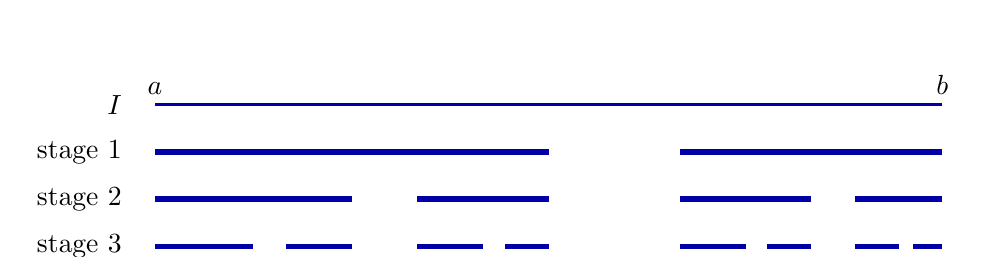
\begin{tikzpicture}[x=10cm,y=.6cm]
 \draw[very thick,blue!65!black] (0,0)--(1,0);
 \node[left] at (-.03,0) {$I$};
 \node[above] at (0,0) {$a$}; \node[above] at (1,0) {$b$};
 \draw[line width=2pt,blue!65!black] (0,-1)--(.5,-1);
 \draw[line width=2pt,blue!65!black] (.6666667,-1)--(1,-1);
 \node[left] at (-.03,-1) {stage 1};
 \draw[line width=2pt,blue!65!black] (0,-2)--(.25,-2);
 \draw[line width=2pt,blue!65!black] (.3333333,-2)--(.5,-2);
 \draw[line width=2pt,blue!65!black] (.6666667,-2)--(.8333333,-2);
 \draw[line width=2pt,blue!65!black] (.8888889,-2)--(1,-2);
 \node[left] at (-.03,-2) {stage 2};
 \draw[line width=2pt,blue!65!black] (0,-3)--(.125,-3);
 \draw[line width=2pt,blue!65!black] (.1666667,-3)--(.25,-3);
 \draw[line width=2pt,blue!65!black] (.3333333,-3)--(.4166667,-3);
 \draw[line width=2pt,blue!65!black] (.4444444,-3)--(.5,-3);
 \draw[line width=2pt,blue!65!black] (.6666667,-3)--(.75,-3);
 \draw[line width=2pt,blue!65!black] (.7777778,-3)--(.8333333,-3);
 \draw[line width=2pt,blue!65!black] (.8888889,-3)--(.9444444,-3);
 \draw[line width=2pt,blue!65!black] (.962963,-3)--(1,-3);
 \node[left] at (-.03,-3) {stage 3};
\end{tikzpicture}
\caption{The logarithmic interval construction, drawn after affine normalization of $I$ to $[0,1]$. Each surviving interval is replaced by its left half and right third.}
\label{fig:cantor}
\end{figure}

\begin{theorem}[Cantor closure]\label{thm:cantor}
Let $\mathcal P=\{\rho_w:w\text{ is nonempty in }F,G\}$. There is a unique nonempty compact set $K\subset I$ satisfying
\[
 K=S_2(K)\cup S_3(K),
\]
and
\begin{equation}\label{eq:closure}
 \overline{\mathcal P}=\exp K.
\end{equation}
This closure is a perfect nowhere dense set of Lebesgue measure zero. Its Hausdorff dimension is the unique positive solution $s$ of
\begin{equation}\label{eq:dimension}
 2^{-s}+3^{-s}=1,
 \qquad s\approx0.7878849110258698.
\end{equation}
The set $\mathcal P$ itself is countable, consists of transcendental numbers, and has Hausdorff dimension zero.
\end{theorem}
\begin{proof}
The maps \eqref{eq:IFS} contract $I$ with ratios $1/2$ and $1/3$ and have disjoint images by \eqref{eq:separation}. The contraction principle for compact subsets gives the unique invariant compact set $K$; equivalently it is the intersection of the nested unions of all image intervals at each word length.

Every finite composition of the $S_i$ has a unique fixed point in $I$. This point lies in $K$: iterate that composition on any point of $K$ and use compactness and invariance. Conversely, each length-$m$ cylinder interval has diameter at most $2^{-m}|I|$ and contains the fixed point of its defining composition. Thus the finite-composition fixed points are dense in $K$.

The inverse of the logarithmic map associated with $T_w$ is a finite composition of the $S_i$ in reversed functional order, with the same fixed point $\log\rho_w$. Reversal permutes the set of finite words, so all finite-composition fixed points arise this way. Exponentiating establishes \eqref{eq:closure}.

The two disjoint branches in every cylinder show that $K$ has no isolated points. The total length of the stage-$m$ union is $(1/2+1/3)^m|I|$, which tends to zero, so $K$ has measure zero and empty interior. It is closed, hence nowhere dense. The strong separation condition permits the standard self-similar dimension theorem \cite{Hutchinson}, giving \eqref{eq:dimension}. Exponentiation is bi-Lipschitz on the compact interval $I$, so it preserves Hausdorff dimension; it also preserves the stated topological properties and the null-set property here. Finally, $\mathcal P$ is countable, and Theorem~\ref{thm:periodic} proves transcendence of every member. Any countable set has Hausdorff dimension zero.
\end{proof}

\begin{remark}
The transcendence conclusion applies to the periodic radii, not to every point of their closure. A limit of transcendental numbers can be algebraic. The positive dimension in \eqref{eq:dimension} belongs to the closure, not to the countable set of periodic radii.
\end{remark}

\section{Scope and further questions}\label{sec:scope}

The results use two distinct arithmetic mechanisms. For ball overlaps, odd-dimensional cap integrals are polynomial, while even-dimensional cap integrals have inverse-trigonometric terms together with a strictly positive algebraic correction. Baker's theorem rules out an algebraic normalized volume for algebraic partial-lens data. For the volume iteration, the argument instead uses the transcendence of $\pi$, multiplicative independence modulo algebraic numbers, and a weighted exponent invariant.

The parity theorem completely classifies inverse overlap radii when the normalized anchor distance and target fraction are algebraic. It does not address arbitrary transcendental anchor data or transcendental target fractions. Nor does odd-dimensional algebraicity alone imply irrationality, a minimal polynomial degree, or nonconstructibility. Proposition~\ref{prop:s4} supplies those additional conclusions only for $\alpha_3$.

Several concrete directions remain. One may seek minimal polynomials and Galois groups for higher odd-dimensional constants, a proof of adjacent-dimensional monotonicity for every $n$, or higher terms and effective error bounds in \eqref{eq:alpha-asympt}. For the iterated maps, it is natural to ask which algebraic numbers, if any, lie in $\exp K$, and to study coefficient families beyond \eqref{eq:MI}. None of these questions is resolved by the density of the periodic radii.

Finally, the exact exceptional-set description in Theorem~\ref{thm:exceptional} identifies what would be required to reach a previously undecided constant $R$. One would need an independent argument locating $R$ relative to the explicit sets $E_w$, or an independent algebraic relation that is incompatible with their classification. Merely substituting the constant into the iteration supplies neither. This separates unconditional results about an entire family from an unsupported claim about one named starting value.

\appendix
\section{Computational checks and reproducibility}

All arithmetic classifications above follow from exact proofs. The numerical values were checked with 65-digit working precision, using bisection on the monotone equation \eqref{eq:half}. For stable evaluation one may use the normalized cap
\[
 H_n(s)=\frac{J_n(s)}{2J_n(0)}
 =\frac12 I_{1-s^2}\!\left(\frac{n+1}{2},\frac12\right)
 \quad(0\leq s\leq1),
\]
where $I_z$ is the regularized incomplete beta function; for negative $s$, use $H_n(-s)=1-H_n(s)$. Then solve
\[
 r^nH_n(r/2)+H_n(1-r^2/2)=\frac12
 \quad\text{on }[0,2].
\]
This special-function notation is only a numerical evaluation device; none of the proofs relies on it. Polynomial expansion of \eqref{eq:half} verifies the displayed odd-dimensional equations. The discriminant and the finite-field factorization in Proposition~\ref{prop:s4} can be checked by exact arithmetic. Bisection of $2^{-s}+3^{-s}-1$ gives \eqref{eq:dimension}. Rounded decimals are illustrative and are not substitutes for the arguments.

\begin{thebibliography}{10}
\bibitem{Baker}
A. Baker, Linear forms in the logarithms of algebraic numbers (III),
\emph{Mathematika} \textbf{14} (1967), no.~2, 220--228.
\href{https://doi.org/10.1112/S0025579300003843}{doi:10.1112/S0025579300003843}.

\bibitem{Finch}
S. R. Finch, \emph{Errata and Addenda to Mathematical Constants},
arXiv:2001.00578v4 (2024), especially Sections 2.33 and 8.2.
\url{https://arxiv.org/html/2001.00578v4}.

\bibitem{Fraser}
M. Fraser, The grazing goat in $n$ dimensions,
\emph{The Two-Year College Mathematics Journal} \textbf{15} (1984), no.~2, 126--134.
\href{https://doi.org/10.1080/00494925.1984.11972761}{doi:10.1080/00494925.1984.11972761}.

\bibitem{HallTenenbaum}
R. R. Hall and G. Tenenbaum, Effective mean value estimates for complex multiplicative functions,
\emph{Mathematical Proceedings of the Cambridge Philosophical Society}
\textbf{110} (1991), no.~2, 337--351.
\href{https://doi.org/10.1017/S0305004100070419}{doi:10.1017/S0305004100070419}.

\bibitem{Hutchinson}
J. E. Hutchinson, Fractals and self similarity,
\emph{Indiana University Mathematics Journal} \textbf{30} (1981), no.~5, 713--747.
\href{https://doi.org/10.1512/iumj.1981.30.30055}{doi:10.1512/iumj.1981.30.30055}.

\bibitem{Meyerson}
M. D. Meyerson, Return of the grazing goat in $n$ dimensions,
\emph{The College Mathematics Journal} \textbf{15} (1984), no.~5, 430--432.
\href{https://doi.org/10.1080/00494925.1984.11972829}{doi:10.1080/00494925.1984.11972829}.

\bibitem{OEIS2}
OEIS Foundation Inc., Entry A133731, planar half-area grazing radius.
\url{https://oeis.org/A133731}. Accessed 12 October 2026.

\bibitem{OEISPsi}
OEIS Foundation Inc., Entry A173201, parameter solving
$2\sin x-2x\cos x=\pi$; see the Hall--Tenenbaum comment and the relation to A133731.
\url{https://oeis.org/A173201}. Accessed 12 October 2026.

\bibitem{OEIS3}
OEIS Foundation Inc., Entry A336198, three-dimensional half-volume grazing radius.
\url{https://oeis.org/A336198}. Accessed 12 October 2026.
\end{thebibliography}
\end{document}
